% !TeX encoding = UTF-8
% chktex-file 21 chktex-file -2 chktex-file 23
\documentclass[fontset=ubuntu,12pt,a4paper,fleqn]{article}
\usepackage[a4paper,left=1cm,right=1cm,top=1cm,bottom=1.5cm,bindingoffset=5mm]{geometry}
\usepackage[UTF8]{ctex}
\usepackage[utf8]{inputenc}
\usepackage[ngerman]{babel}
\usepackage{amsmath}
\usepackage{amsfonts}
\usepackage{amssymb}
\usepackage{commath}
\usepackage{tikz}
\usepackage{pgfplots}
\usepackage{helvet}
\usepackage{tabu}
\usepackage{multicol}
\usepackage[pdftex,pdfa,hidelinks]{hyperref}
\usepackage[autostyle=true,german=quotes]{csquotes}

\setlength{\parindent}{0em} 
\pagenumbering{arabic}

\begin{document}

{\Large\textbf{Matrizenmultiplikation mit dem Falkschema}\par}

\setlength{\columnseprule}{0.4pt}
\begin{multicols}{2}

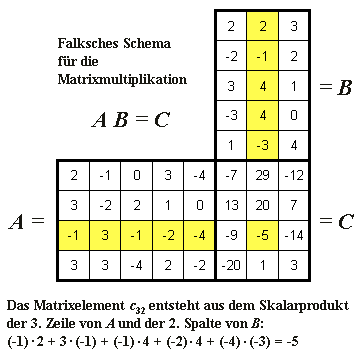
\includegraphics[width=0.7\linewidth]{FalkschesSchema.png}

{\Large\textbf{Einfache Ableitungsregeln}\par}

\textbf{Faktroregel:}
\[
y= C\cdot f(x) \Rightarrow y'= C\cdot f'(x)
\]
\textbf{Summenregel:}
\[
y= f_1(x) + f_2(x) + ... + f_n(x)  
\]\[
\Rightarrow y'=f'_1(x) + f_2'(x) + ... + f_n'(x)
\]
\textbf{Produktregel:}
\[
y= u(x) \cdot v(x) \Rightarrow y'=u'(x) \cdot v(x) + u(x) \cdot v'(x)
\]
\textbf{Quotientenregel:}
\[
y= \frac{u(x)}{v(x)} \Rightarrow y'=\frac{u'(x) \cdot v(x) - u(x) \cdot v'(x)}{[v(x)]^2}
\]
\textbf{Kettenregel:}
\[
y=a(b(c(x))) \Rightarrow y'= a'(x) \cdot b'(x) \cdot c'(x)
\]

\textbf{Wichtige Ableitungen:}
\begin{align*}
	f(x) &\Rightarrow f'(x)\\
	\ln(x) &\Rightarrow \frac{1}{x}\\
	\arccos(x) &\Rightarrow -\frac{1}{\sqrt{1-x^2}}\\
\end{align*}

\textbf{Wichtige Rechnungen:}
\begin{align*}
	\ln(1) &=0
\end{align*}
\newpage
\end{multicols}






{\Large\textbf{Partielle Ableitungen}\par}

\textbf{Bildung partieller Ableitungen:}
Die partiellen Ableitungen einer Funktion $f(x_1,x_2,x3)= x_1\cdot x_2+x3$ lassen sich sich wie folgt bestimmen:
\begin{align*}
\frac{\partial f}{\partial x_1}(x_1,x_2,x_3) &= 1\cdot x_2\\
\frac{\partial f}{\partial x_2}(x_1,x_2,x_3) &= x_1\cdot 1\\
\frac{\partial f}{\partial x_3}(x_1,x_2,x_3) &= 1
\end{align*}

\textbf{Berechnung der Tangentialebene:}
Es seien \(\mathbb{D} \subset \mathbb{R}^2, f:\mathbb{D}->\mathbb{R}\) eine partiell differenzierbare Funktion und \((x_{01},x_{02})\in\mathbb{D}\). Dann lautet die Gleichung der Tangentialebene für den Punkt \((x_{01},x_{02})\):

\begin{align*}
x_3&=f(x_{01},x_{02})+\dpd{f}{x_1}(x_{01},x_{02})(x_1-x_{01})+\dpd{f}{x_2}(x_{01},x_{02})(x_2-x_{02})\\
&=f(x_{01},x_{02})+\begin{pmatrix} \dpd{f}{x_1} (x_{01},x_{02}) & \dpd{f}{x_2}(x_{01},x_{02}) \end{pmatrix} \cdot \begin{pmatrix} (x_1-x_{01})\\ (x_2-x_{02}) \end{pmatrix}
\end{align*}

Zuerst den Punkt $(x_{01},x_{02})$ an den Stellen $x_{01}$ und $x_{02}$ einsetzen. Dann ausrechnen und am Ende den Punkt für  $x_{1}$ und $x_{2}$ einsetzen um zum Ergebnis für x3 an dem genannten Punkt zu kommen.\\

\textbf{Berechnung Gradient:}
Es sei \(\mathbb{D} \subset \mathbb{R}^n\) und \(f:\mathbb{D} \to \mathbb{R}\) partiell differenzierbar. Dann heißt der Vektor \(\mathrm{grad} f(x) = \begin{pmatrix}
\dpd{f}{x_1}(x) \\
\dpd{f}{x_2}(x) \\
\vdots \\
\dpd{f}{x_n}(x) \\
\end{pmatrix}\) der Gradient von \(f\) im Punkt \(x\in\mathbb{D}= (x_1,\dots,x_n)\).\\Anstelle von \(\mathrm{grad} f(x)\) wird auch häufig \(\nabla f(x)\) geschrieben.\\

\textbf{Partielle Ableitungen k-ter Ordnung:}

Es sei \(D\subset\mathbb{R}^n,f:D\to\mathbb{R}\) eine partiell differenzierbare Funktion und \(x_0 \in D\). Die Funktion f heißt \\ zweimal \textbf{partiell differenzierbar} in \(x_0\), wenn alle partiellen Ableitungen \(\pd{f}{x_i}\) in \(x_0\) wieder partiell differenzierbar sind.

Man schreibt \(\frac{\partial^2 f}{\partial x_j x_i}(x_0)=\pd{}{x_j}\left(\pd{f}{x_i}\right)(x_0)=f_{x_j x_i}(x_0)\)

Dieser Ausdruck heißt dann \textbf{zweite partielle Ableitung} von f.

Allgemein heißt f \textbf{k-mal partiell differenzierbar}, wennn alle (k-1)-ten partiellen Ableitungen von f wieder partiell differenzierbar sind. Man schreibt:

\[\dpd{f}{x_{ik} \partial x_{i(k-1)} \dots \partial x_{i1}}(x_0) = \frac{\partial}{\partial x_{ik}}\left(\frac{\partial^{k-1} f}{\partial x_{i(k-1)} \dots \partial x_{i1}}\right)(x_0)=f_{x_{ik} \dots x_{i1}}\]

\textbf{Satz von Schwarz:}
Es sei \(D\subset\mathbb{R}^n,f:D\to\mathbb{R}\) zweimal stetig partiell differenzierbar. Dann ist \(\frac{\partial^2 f}{\partial x_i \partial x_j}=\frac{\partial^2 f}{\partial x_j \partial x_i}\) für alle \(i,j\in\left\{1,\dots,n\right\}\). Die Reihenfolge der Ableitungsvariablen spielt also keine Rolle.
\newpage








{\Large\textbf{Totale Differenzierbarkeit}\par}
\textbf{Vektorfunktion:}
Eine eindeutige Abbildung \(f:\mathbb{D}\to W,\mathbb{D}\subset\mathbb{R}^n,W\subset\mathbb{R}^m,m>1\) mit mehrdimensionalem Wertebereich heißt \underline{Vektorfunktion}.
     
\begin{multicols}{2}
\textbf{Beispiel:}
Es sei \(\mathbb{D}\subset\mathbb{R}^3\to\mathbb{R}^2\) gegeben durch
\[f(x_1,x_2,x_3)=\begin{pmatrix}
x_1+x_3 \\ x_2+x_3
\end{pmatrix}\]
$f(x_1,x_2,x_3)$ hat 2 Ergebniskomponenten:
\[f_1(x_1,x_2,x_3)=x_1+x_2\]
\[f_2(x_1,x_2,x_3)=x_2+x_3\]
\end{multicols}

\begin{multicols}{2}
\textbf{Jacobi-Matrix:}
Es sei \(f:\mathbb{D}\to \mathbb{R}^m,\mathbb{D}\subset\mathbb{R}^n\) eine Abbildung und \(x_0\in\mathbb{D}\). Weiterhin sei f in \(x_0\) total differenzierbar mit der Matrix
\[A=(a_{ij});i=1,\dots,m;j=1,\dots,n \in\mathbb{R}^{m\times n}\]
Dann ist f in \(x_0\) stetig und alle Komponentenfunktionen \(f_1,\dots,f_m:\mathbb{R}^n\to\mathbb{R}\) sind in \(x_0\) partiell differenzierbar, wobei gilt: \(a_{ij}=\pd{f_i}{x_j}(x_0)\).\\
Die Matrix heißt Funktionalmatrix oder auch Jacobi-Matrix von f und wird mit \(Df(x_0)\) oder \(J_f(x_0)\) bezeichnet.
\[Df(x_0)=\begin{pmatrix}
\dpd{f_1}{x_1}(x_0) & \dpd{f_1}{x_2}(x_0) & \cdots & \dpd{f_1}{x_n}(x_0) \\
\dpd{f_2}{x_1}(x_0) & \dpd{f_2}{x_2}(x_0) & \cdots & \dpd{f_2}{x_n}(x_0) \\
\vdots & \vdots & \ddots & \vdots \\
\dpd{f_m}{x_1}(x_0) & \dpd{f_m}{x_2}(x_0) & \cdots & \dpd{f_m}{x_n}(x_0)
\end{pmatrix}\]
\end{multicols}
\textbf{Totale Differenzierbarkeit}
Sei \(f:\mathbb{R}^2\to\mathbb{R}\) eine total differenzierbare Funktion. Dann kann f in der Nähe eines Punktes \((x_{01},x_{02})\in\mathbb{R}^2\) durch \(f(x_{01},x_{02})+Df(x_{01},x_{02})\begin{pmatrix}x_1-x_{01} \\ x_2-x_{02}\end{pmatrix}\) angenähert werden.

Es gilt also \(f(x_1,x_2)=f(x_{01},x_{02})+\begin{pmatrix}
\dpd{f}{x_1}(x_{01},x_{02}) & \dpd{f}{x_2}(x_{01},x_{02})\end{pmatrix}\begin{pmatrix}
x_1-x_{01} \\ x_2-x_{02}
\end{pmatrix}\)

\[f(x_1,x_2)-f(x_{01},x_{02})\approx\dpd{f}{x_1}(x_{01},x_{02})\cdot\underbrace{(x_1-x_{01})}_{=:\Delta x_1} + \dpd{f}{x_2}(x_{01},x_{02})\cdot\underbrace{(x_2-x_{02})}_{=:\Delta x_2}\]

also gilt: \(\Delta f\approx \pd{f}{x_1}\cdot\Delta x_1 + \pd{f}{x_2}\cdot\Delta x_2\)

Für \enquote{beliebig kleines} \(\Delta x_1\) und \(\Delta x_2\) schreiben wir \enquote{d} statt \enquote{\(\Delta\)} und \enquote{=} statt \enquote{\(\approx\)}.

\[\boxed{df = \dpd{f}{x_1}(x_{01},x_{02})\cdot dx_1 + \dpd{f}{x_2}(x_{01},x_{02})\cdot dx_2} \]
Diesen Ausdruck bezeichnet man als \underline{totales Differenzial} der Funktion f.

Für eine Funktion \(f:\mathbb{R}^n\to\mathbb{R}\) gilt:
\[\boxed{df = \dpd{f}{x_1}\cdot dx_1 + \dpd{f}{x_2}\cdot dx_2 + \cdots + \dpd{f}{x_2}\cdot dx_n}\]



    
\end{document}  